\chapter{Μετρήσεις και Επίδειξη Συστήματος}
\label{chapter:system_showcase}

Στο κεφάλαιο αυτό θα μελετήσουμε την απόδοση του συστήματος Lychte που υλοποιήσαμε στο πλαίσιο της διπλωματικής
αυτής εργασίας και στο τέλος θα παρουσιαστούν εικόνες από τη γραφική διεπαφή, την εφαρμογή δηλαδή που αναπτύξαμε.

\section{Μετρήσεις}
\label{section:expreriments}

Προκειμένου να παρακολουθήσουμε τις ανάγκες και να δοκιμάσουμε τα όρια του Lychte καναμε μία σειρά διαφορετικών μετρήσεων. Η παράμετρος
που αλλάζει σε κάθε μέτρηση είναι ο αριθμός των Apis/Jobs που τρέχει παράλληλα ένας worker. Έτσι σε κάθε διαφορετική μέτρηση
κάναμε n καταχωρήσεις Apis και Jobs αντίστοιχα, όπου n o αρθμός των αιτημάτων που θέλουμε να ελέγχουμε. Στο σημείο αυτό πρέπει να ανεφερθεί
ότι οι μετρήσεις έγιναν σε μηχάνημα με τα εξής τεχνικά χαρακτηριστικά:

\begin{table}[H]
	\begin{center}
		\caption{Τεχνικά χαρακτηριστικά Υπολογιστικού Συστήματος}
		\label{tab:pc_specs}
		\begin{tabular}{| c | c |}
			\hline
			\thead{Operating System} & WindowsOS                  \\
			\hline
			\thead{Processor}        & AMD Ryzen 7 5800H (3.2Ghz) \\
			\hline
			\thead{RAM}              & 16GB                       \\
			\hline
		\end{tabular}
	\end{center}
\end{table}

\subsection{Περιγραφή}
\label{subsection:experiment_summary}

ΓΡΑΨΕ ΓΙΑ ΤΟ ΤΡΟΠΟ ΠΟΥ ΜΠΗΚΑΝ ΤΑ APIS ΣΤΗ ΒΑΣΗ (ΜΕΤΑΞΎ 8 APIS ΕΠΙΛΕΟΝΤΑΝ ΕΝΑ ΣΤΗΝ ΤΥΧΗ ΜΕ INTERVAL 0.5 Ή 1 Ή 2 Ή 3)

ΑΝΑΦΕΡΕ ΌΤΙ ΑΥΤΆ ΑΦΟΡΟΎΝ ΤΙΣ ΤΕΛΕΥΤΑΙΕΣ ΤΡΕΙΣ ΩΡΕΣ ΛΕΙΤΟΥΡΓΙΑΣ, Ή ΟΤΙ ΑΝΑΦΕΡΟΝΤΑΙ ΣΕ ΤΡΕΙΣ ΩΡΕΣ ΛΕΙΤΟΥΡΓΙΑ ΓΕΝΙΚΑ
MΈΤΡΗΣΗ ΚΆΘΕ ΤΡΙΆΝΤΑ ΔΕΥΤΕΡΟΛΕΠΤΑ

\begin{figure}[!ht]
	\centering
	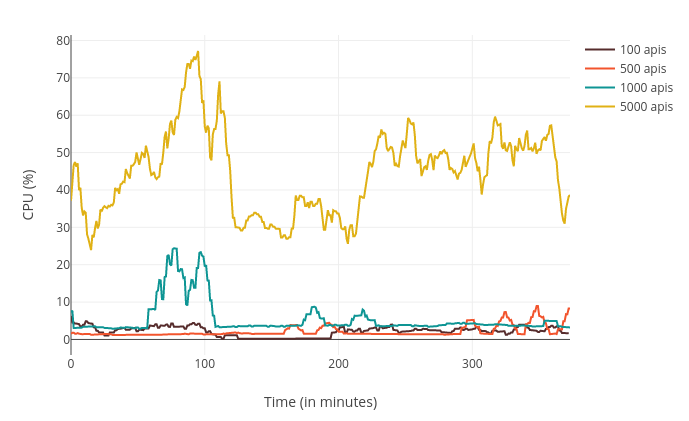
\includegraphics[width=0.8\textwidth]{./images/chapter5/cpu-plot.png}
	\caption[Αποτελέσματα χρήσης της CPU]{Αποτελέσματα χρήσης της CPU}
	\label{fig:cpu_usage}
\end{figure}

\begin{figure}[!ht]
	\centering
	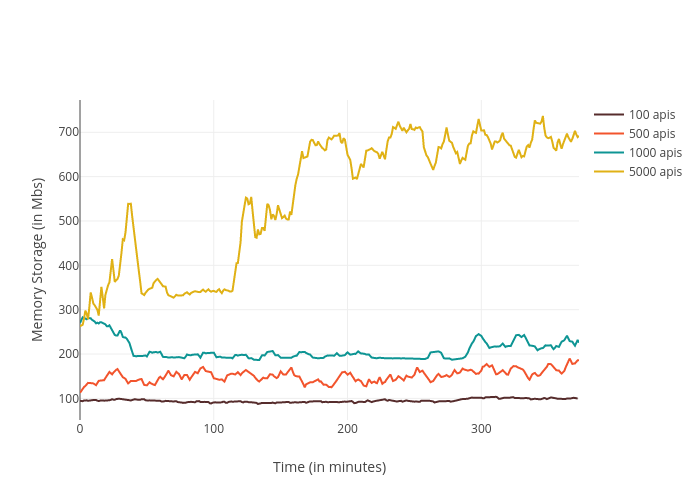
\includegraphics[width=0.8\textwidth]{./images/chapter5/memory-plot.png}
	\caption[Αποτελέσματα χρήσης της RAM]{Αποτελέσματα χρήσης της RAM}
	\label{fig:ram_usage}
\end{figure}

ΓΕΝΙΚΆ ΣΤΑΤΙΙΣΤΙΚΑ ΑΠΌ ΤΑ ΠΑΡΑΠΑΝΩ ΣΕ ΜΕΓΑΛΎΤΕΡΟ ΒΑΘΟΣ ΧΡΟΝΟΥ (12 ΩΡΕΣ)

\begin{table}[H]
	\begin{center}
		\caption{Αποτελέσματα Μετρήσεων}
		\label{tab:results}
		\begin{tabular}{| c | c | c | c |}
			\hline
			                  & \thead{Μέση Απόκλιση} & \thead{Μέση Χρήση CPU} & \thead{Μέση Χρήση RAM} \\
			\hline
			\thead{100 apis}  & -112.62ms             & 1.22\%                 & 102.54Mb               \\
			\hline
			\thead{500 apis}  & -69.32ms              & 3.26\%                 & 171.1Mb                \\
			\hline
			\thead{1000 apis} & -47.9ms               & 7.46\%                 & 223.13Mb               \\
			\hline
			\thead{5000 apis} & 664ms                 & 56.36\%                & 652.45Mb               \\
			\hline
		\end{tabular}
	\end{center}
\end{table}


\begin{figure}[!ht]
	\centering
	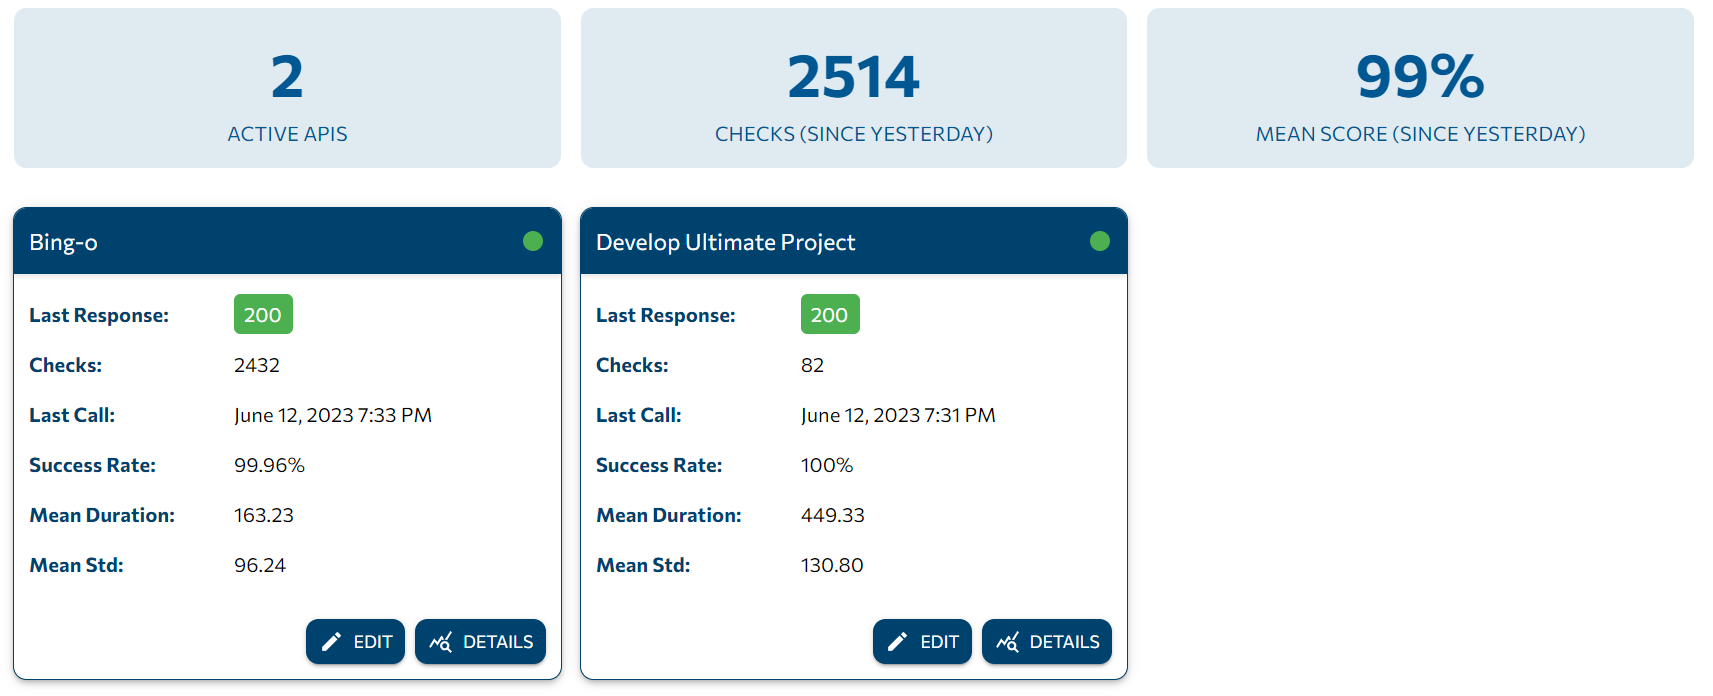
\includegraphics[width=0.8\textwidth]{./images/chapter5/overview_landing.png}
	\caption[Lychte Api Overview]{Lychte Api Overview}
	\label{fig:lychte_overview}
\end{figure}

\begin{figure}[!ht]
	\centering
	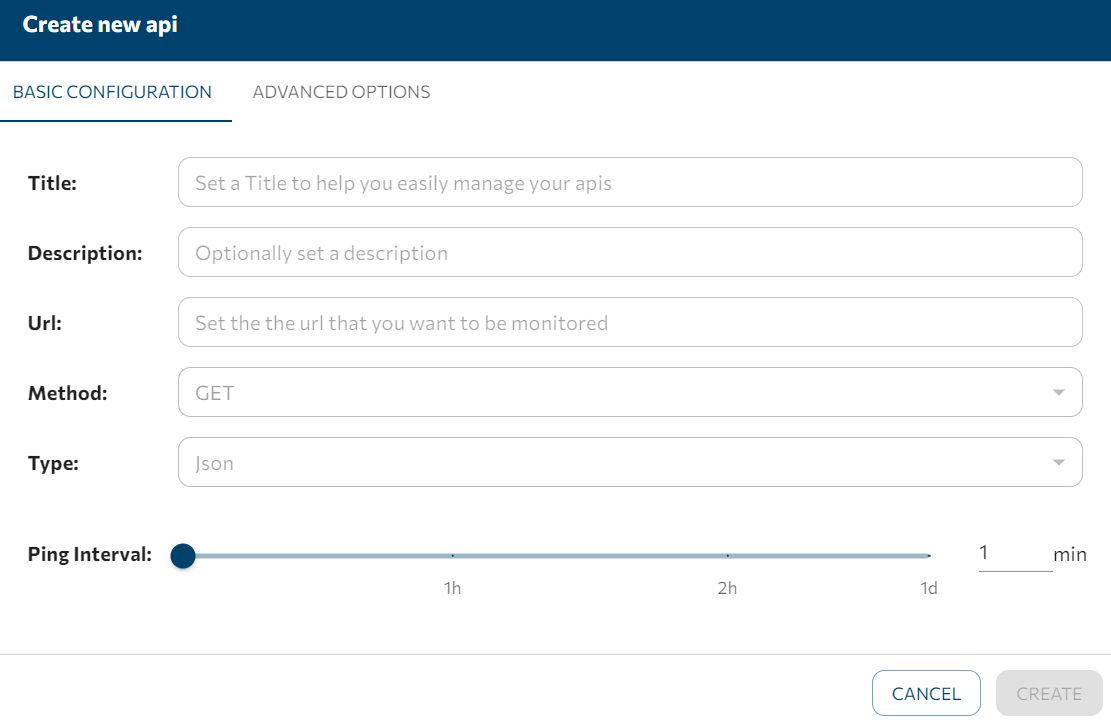
\includegraphics[width=0.8\textwidth]{./images/chapter5/api_creation.png}
	\caption[Lychte Create Api Check]{Lychte Create Api Check}
	\label{fig:lychte_create_api}
\end{figure}

\begin{figure}[!ht]
	\centering
	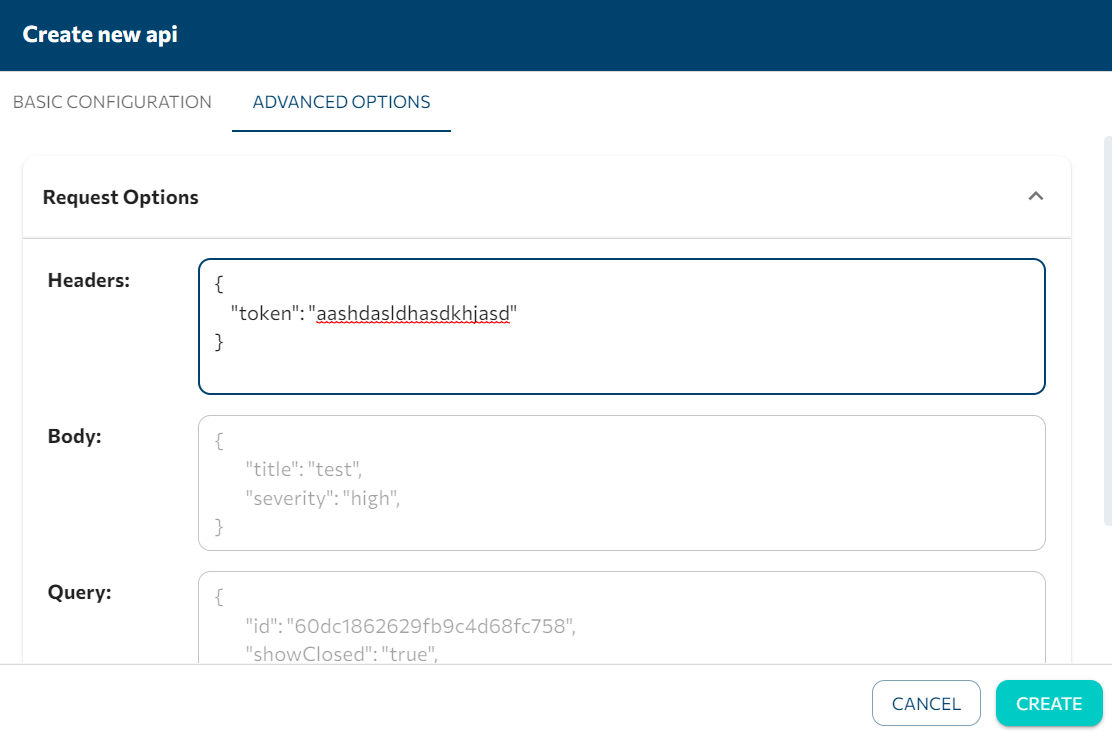
\includegraphics[width=0.8\textwidth]{./images/chapter5/api_creation_advanced_features.png}
	\caption[Lychte Create Api Advanced Check]{Lychte Create Api Advanced Check}
	\label{fig:lychte_create_advanced_api}
\end{figure}

\begin{figure}[!ht]
	\centering
	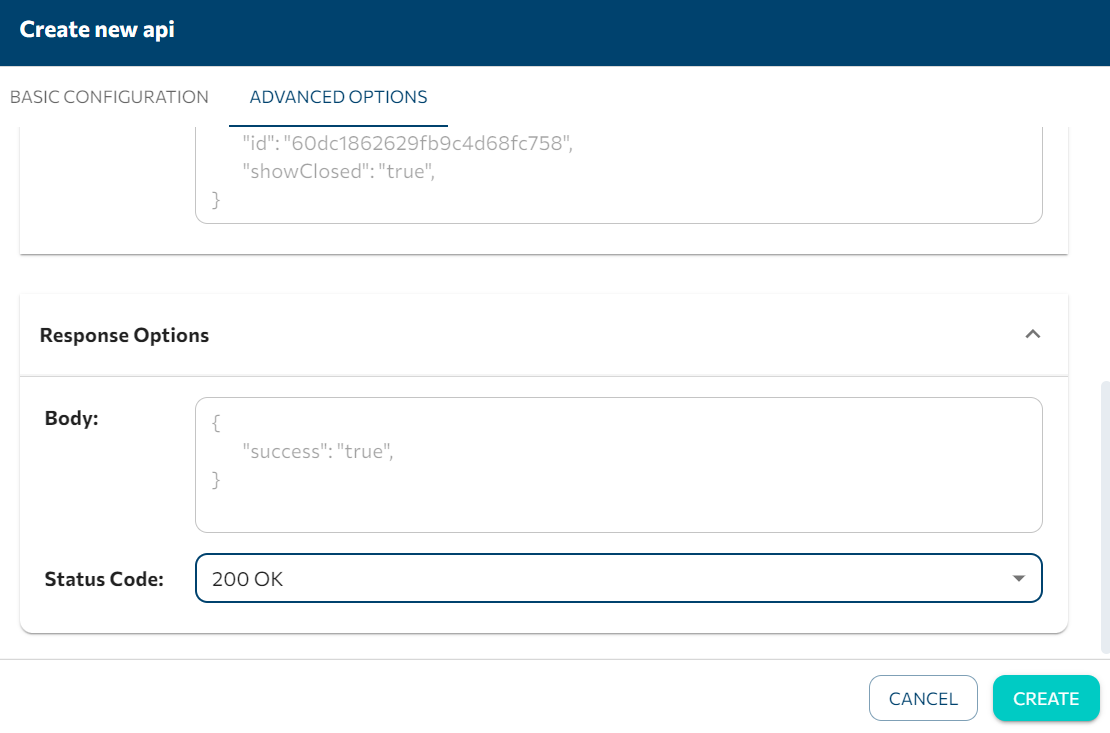
\includegraphics[width=0.8\textwidth]{./images/chapter5/api_creation_advanced_features_v2.png}
	\caption[Lychte Create Api Advanced v2 Check]{Lychte Create Api Advanced v2 Check}
	\label{fig:lychte_create_advanced_v2_api}
\end{figure}

\begin{figure}[!ht]
	\centering
	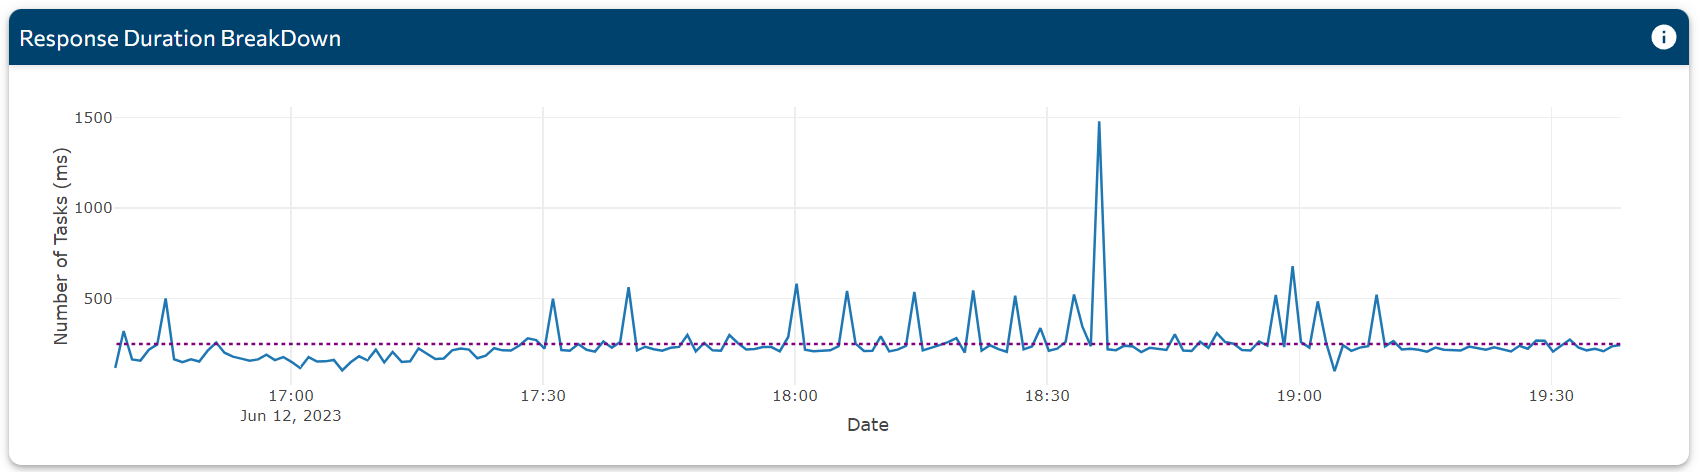
\includegraphics[width=0.8\textwidth]{./images/chapter5/response_duration_breakdown.png}
	\caption[Διάγραμμα Διάρκειας Αποκρίσεων]{Διάγραμμα Διάρκειας Αποκρίσεων}
	\label{fig:lychte_response_duration_breakdown}
\end{figure}

\begin{figure}[!ht]
	\centering
	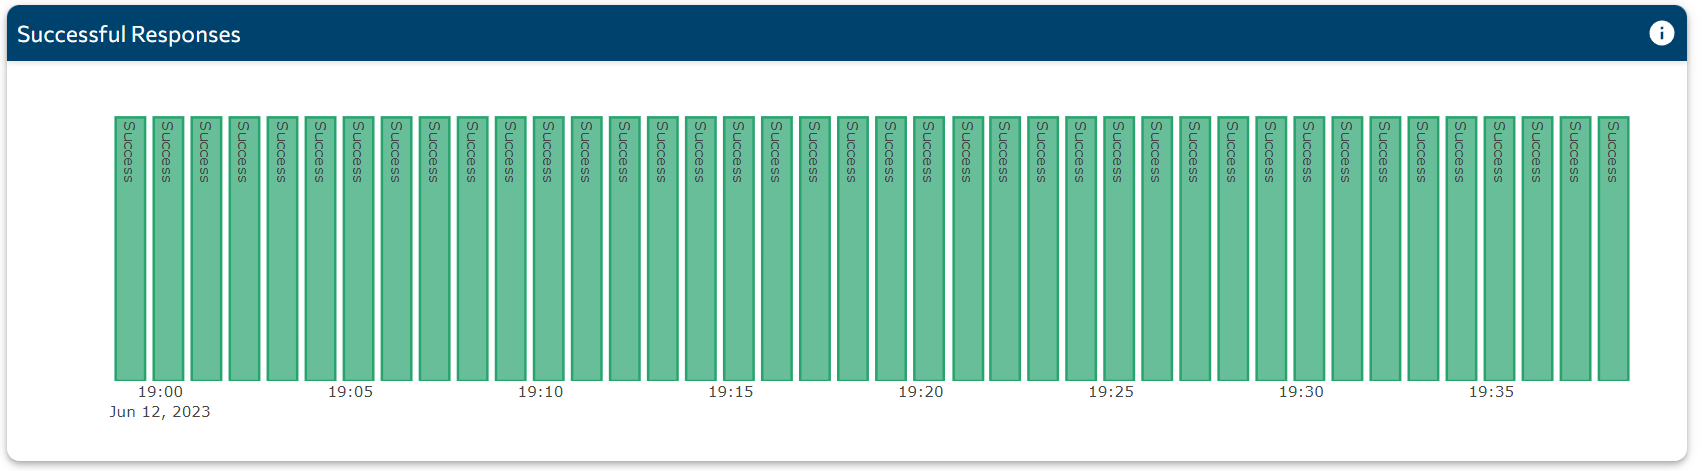
\includegraphics[width=0.8\textwidth]{./images/chapter5/succesfull_responses.png}
	\caption[Διάγραμμα Κατάστασης Αποκρίσεων]{Διάγραμμα Κατάστασης Αποκρίσεων}
	\label{fig:lychte_succesfull_responses}
\end{figure}

\begin{figure}[!ht]
	\centering
	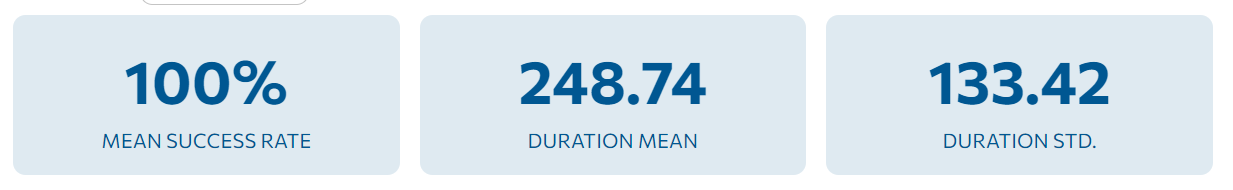
\includegraphics[width=0.8\textwidth]{./images/chapter5/metrics.png}
	\caption[Μετρικές που αφορούν το σύνολο των δεδομένων (ιστορικά δεδομένα)]{Μετρικές που αφορούν το σύνολο των δεδομένων (ιστορικά δεδομένα)}
	\label{fig:lychte_metrics}
\end{figure}

\begin{figure}[!ht]
	\centering
	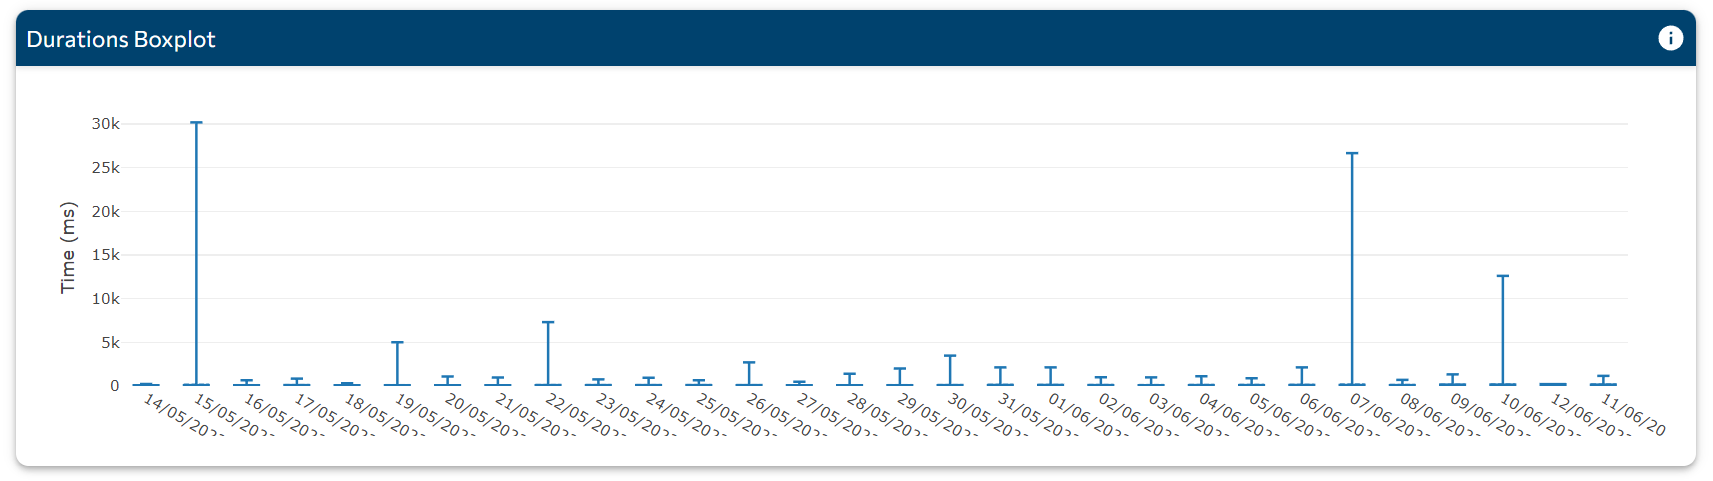
\includegraphics[width=0.8\textwidth]{./images/chapter5/duration_boxplot_diagram.png}
	\caption[Διάγραμμα Θηκογραμμάτων (Boxplots) της διάρκειας απόκρισης αιτημάτων για κάθε μέρα (ιστορικά δεδομένα)]{Διάγραμμα Θηκογραμμάτων (Boxplots) της διάρκειας απόκρισης αιτημάτων για κάθε μέρα (ιστορικά δεδομένα)}
	\label{fig:lychte_boxplot}
\end{figure}
